\documentclass{article}
\PassOptionsToPackage{numbers, compress}{natbib}
\usepackage{pnpl_2026_competition}
\usepackage[utf8]{inputenc}
\usepackage[T1]{fontenc}
\usepackage{hyperref}
\usepackage{url}
\usepackage{booktabs}
\usepackage{amsfonts}
\usepackage{amsmath}
\usepackage{nicefrac}
\usepackage{microtype}
\usepackage{xcolor}
\usepackage{graphicx}

\title{When the Public Leaderboard Misleads:\\ Lessons from 99 Scored Submissions in Single-Subject MEG Word Decoding}

\author{%
  Tun-Yu Kuo \\
  Independent Researcher \\
  \texttt{kuotunyh@gmail.com} \\
  Kaggle team: \texttt{yu\_kuo14}
}

\begin{document}
\maketitle

\begin{abstract}
We describe our Deep-track entry to the 2026 PNPL Competition. The task is to decode which of 50 common English words a participant hears from magnetoencephalography (MEG), scored by class-balanced top-10 accuracy (BAcc@10). Our system combines an ensemble of convolutional word encoders and sentence-level Transformers with a closed-vocabulary language-model (LM) prior.

In the last week we added two language-side components: an LM fine-tuned on synthetic vocabulary-only sentences, and whole-sentence candidate decoding. They raised our public score to 0.733, 13th of 90 teams on the public leaderboard of 20 October. On the private leaderboard our final selection scored 0.663, 44th of 91 teams on 25 October. Our best private score among all submissions, 0.688, came from a simpler system submitted a week earlier.

Kaggle revealed private scores for all 99 of our submissions, and each submission's change is recorded, so we can examine this gap after the fact. In 30 reference--variant comparisons, changes with an absolute public effect of at least 0.03 kept their sign on the private split in 6 of 8 cases; smaller changes kept it in only 8 of 22. Among the 60 pre-deadline submissions with public score at least 0.66, public and private scores were negatively correlated ($r=-0.37$). When our in-session validation disagreed with the public score, neither was clearly better (4 of 8 each). But the cost was asymmetric: following validation would have gained up to 0.022 and lost at most 0.010. Selecting the ten best public submissions did worse than all but 0.24\% of random selections from the same pool.

These are exploratory observations from one development history. We report them with the system and draw practical recommendations for model selection on small public splits.
\end{abstract}

\section{Introduction}

Each test item is a word heard by \texttt{subj0}, either within a sentence or in isolation. A system outputs a distribution over the 50 target words, and the score is the mean over the 50 words of each word's Recall@10 (chance 0.20). The training data are about 780k words of audiobooks, TIMIT, MOCHA-TIMIT and podcasts. The test sentences are short conversational utterances composed almost entirely of the 50 target words~\cite{pnpl2026}.

During the competition, Kaggle shows a public score computed on part of the test set; the private score is revealed afterwards. We relied heavily on the public score, submitting up to ten times a day, which exposed us to adaptive over-selection on a small public split. Because private scores were later released for all of our submissions, we can look back at how public and private scores related.

The paper has three parts: the system (Section~\ref{sec:system}), a retrospective public--private analysis (Section~\ref{sec:analysis}), and a back-test of final-selection rules with recommendations (Section~\ref{sec:selection}). All leaderboard statistics are computed from the Kaggle export of our submissions by a released script. Experimental settings and the selection history come from our dated experiment log.

\section{System}
\label{sec:system}

\begin{figure}[t]
  \centering
  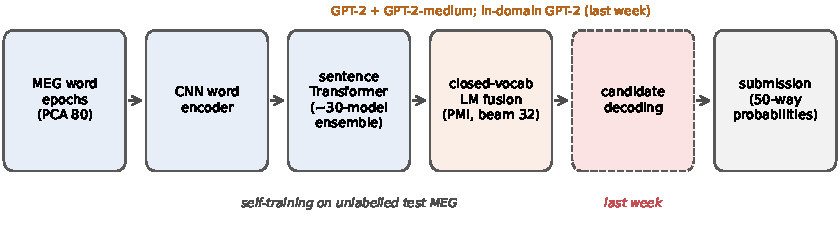
\includegraphics[width=\linewidth]{fig_system.pdf}
  \caption{System overview. Dashed: whole-sentence candidate decoding, added in the last week together with the in-domain GPT-2.}
  \label{fig:system}
\end{figure}

Figure~\ref{fig:system} gives an overview.

\paragraph{Data and validation.} Each run is z-scored per channel and projected by a global, whitened PCA from 306 to 80 components. Word epochs span $[-0.5, 2.5]$\,s at 50 or 100\,Hz (``3\,s'' models) or $[0, 1]$\,s at 125\,Hz (``1\,s'' models). TIMIT SA1/SA2 sentences recur 630 times each, and sentence models memorise them. We therefore train repeated sentences as isolated words and validate on held-out sentences whose text never occurs in training.

Validation uses seven runs held out from the training sessions. The test recordings were made separately, and their per-component input scale is about 1.35 times that of training. From the held-out runs we also built a proxy of the test set: 1{,}042 target words in 312 segments, restricted to the 50 words.

\paragraph{MEG decoder.} We follow the word-decoding setup of d'Ascoli et al.~\cite{dascoli2025}, without their semantic objective. A convolutional encoder maps each word epoch to an embedding, and a pre-norm Transformer over the words of a sentence classifies each word among 1{,}000 classes. The base configuration has $d{=}512$ and 8 layers; a second head classifies each word without context. Final ensembles average the log-probabilities of about 30 members, which differ in window, sampling rate, depth (8 to 16 layers), CNN width and input normalisation. Some members are self-trained on the unlabelled test recordings with soft targets from an earlier submission.

\paragraph{Language prior.} A causal LM gives a next-word score for each of the 50 words, using the beam hypotheses as context. We subtract the log of its average probability over all test sentence positions (PMI) and add the result to the MEG log-probabilities with weight 0.5. The beam size is 32, and GPT-2~\cite{radford2019} and GPT-2-medium are combined after matching the spread of their PMI terms. In the last week we added two components:
\begin{itemize}
\item \emph{In-domain LM.} GPT-2 is fine-tuned on 807 to 3{,}742 synthetic sentences that use only the 50 words, written by Claude and Qwen3.5-9B~\cite{qwen35}.
\item \emph{Whole-sentence candidate decoding.} Every length-matched candidate sentence is scored against the MEG evidence at all positions, and the resulting per-position marginals are mixed into the submission. The recipe of our best public submission adds LLM proposals prompted with our top-6 words per position, an LM prior (0.5 times the candidate's in-domain LM log-probability) and mixing weight 0.3. A simpler variant uses generic candidates only, mixing weight 0.15 and no LM prior.
\end{itemize}

\paragraph{Isolated words.} For the 92 isolated words we averaged the contextual and context-free heads and applied a prior correction ($\tau=0.7$). During the competition we assumed these rows counted only towards the private score. In fact, in four pairs of submissions that differed only in these rows, both the public and the private scores were identical to five decimals, although in the three pairs whose files we kept, 33--82\% of these rows had different top-10 sets. These rows therefore appear not to be scored in either split, and our tuning of them had no effect.

\section{Public versus private}
\label{sec:analysis}

\begin{figure}[t]
  \centering
  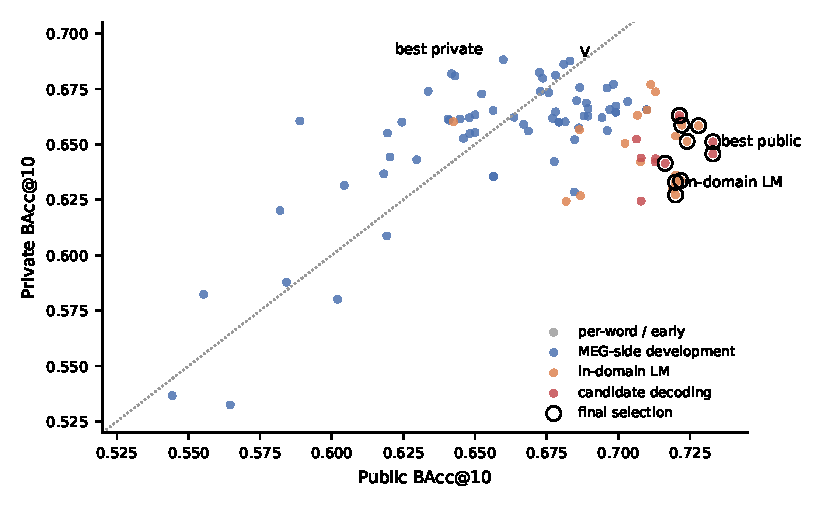
\includegraphics[width=0.84\linewidth]{fig_scatter.pdf}
  \caption{Public and private BAcc@10 of our submissions with public score at least 0.5 (dotted line: equal scores). Circles mark the ten submissions in our final selection. V is the validation-motivated stack.}
  \label{fig:scatter}
\end{figure}

\begin{figure}[t]
  \centering
  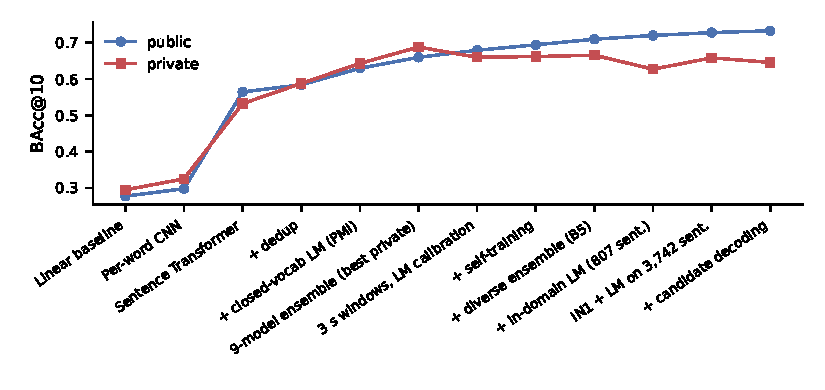
\includegraphics[width=0.84\linewidth]{fig_progression.pdf}
  \caption{Selected development milestones on the public and private splits, including the 9-model ensemble that has our best private score. Each milestone may change several components.}
  \label{fig:progression}
\end{figure}

Figures~\ref{fig:scatter} and~\ref{fig:progression} summarise the outcome. Over the 95 pre-deadline submissions, public and private scores correlate at $r=0.92$, but this mostly reflects the large early steps. The correlation falls to $0.50$ once the four sub-0.5 baselines are excluded. It becomes negative among the 60 submissions with public score at least 0.66 ($r=-0.37$) and among the 32 with at least 0.69 ($r=-0.53$).

Our best private score, 0.6881, came from a 9-model ensemble with GPT-2 fusion submitted on 9 October (public 0.660); no later submission exceeded it. The 25 pre-deadline language-side submissions averaged 0.711 public but 0.648 private, against 0.658 and 0.654 for the 66 MEG-side submissions before them.

These patterns are consistent with over-selection on the public split. Most later submissions branched from whichever submission had just reached a public peak, so their public scores were partly selected noise, and their private scores regressed. A single development history cannot separate this from genuine public/private differences.

\begin{table}[t]
  \caption{Selected reference--variant comparisons: change in public and private score, and what in-session validation suggested before the private release ($+$ helps, $-$ hurts, n/a no matched validation result documented). $^\dagger$ marks bundles of several changes. All 30 comparisons are listed in Appendix~\ref{app:pairs}.}
  \label{tab:pairs}
  \centering
  \small
  \begin{tabular}{lrrc}
    \toprule
    Change (variant minus reference) & $\Delta$ public & $\Delta$ private & Validation \\
    \midrule
    sentence-context model (redesign)$^\dagger$ & $+0.267$ & $+0.207$ & n/a \\
    closed-vocab LM fusion (PMI) & $+0.045$ & $+0.055$ & $+$ \\
    Qwen3-8B instead of GPT-2 & $-0.041$ & $-0.079$ & $-$ \\
    LM fusion without PMI (N-best)$^\dagger$ & $-0.074$ & $-0.061$ & n/a \\
    \midrule
    self-training round 1 & $+0.015$ & $+0.002$ & n/a \\
    LM fusion after self-training & $+0.022$ & $-0.012$ & n/a \\
    all members self-trained (one teacher)$^\dagger$ & $-0.014$ & $-0.049$ & n/a \\
    sentence-end LM term & $-0.051$ & $+0.019$ & n/a \\
    sentence prior correction $\tau{=}0.3$ & $-0.037$ & $+0.017$ & $+$ \\
    word-timing evidence $\beta{=}0.5$ & $-0.060$ & $-0.010$ & $+$ \\
    validation-motivated stack V$^\dagger$ & $-0.027$ & $+0.022$ & $+$ \\
    \midrule
    in-domain LM (807 sentences, seed 0) & $+0.010$ & $-0.038$ & n/a \\
    in-domain LM, 3-seed mixture$^\dagger$ & $+0.010$ & $-0.012$ & n/a \\
    in-domain corpus 807 $\to$ 1,368 & $-0.010$ & $+0.038$ & n/a \\
    in-domain corpus 807 $\to$ 2,103 (+ Qwen sentences; IN1) & $+0.002$ & $+0.018$ & n/a \\
    generic candidates, $\lambda{=}0.15$ & $-0.003$ & $+0.012$ & n/a \\
    candidate decoding (guided pool + LM prior)$^\dagger$ & $+0.009$ & $-0.006$ & n/a \\
    \bottomrule
\end{tabular}

\end{table}

\paragraph{Paired comparisons.} We specified 30 reference--variant comparisons between submissions; 17 isolate one documented change and 13 bundle several (Table~\ref{tab:pairs}, Figure~\ref{fig:pairs}a, Appendix~\ref{app:pairs}). Changes with an absolute public effect of at least 0.03 kept their sign on the private split in 6 of 8 cases. Smaller changes kept it in only 8 of 22 (Wilson 95\% interval 0.20--0.57), and the correlation of their public and private effects was $-0.31$. The pattern is similar with thresholds of 0.025 or 0.035 and when only single changes are counted (5 of 11 small changes). The comparisons share baselines and were chosen by us, so these figures describe our history rather than a calibrated threshold.

The language components show the selection problem clearly. Replacing GPT-2 with the 807-sentence in-domain LM gained $+0.010$ public but lost $0.038$ private. Expanding the corpus to 1{,}368 or 2{,}103 sentences \emph{raised} the private score by $0.038$ and $0.018$, while the public score fell or barely moved. Across in-domain-LM submissions the private score ranged from 0.624 to 0.677, and the variants with the highest public scores were among the lowest on private. Likewise, generic candidates gained $+0.012$ private, while the guided-pool recipe with the LM prior, which had the best public score, lost $0.006$.

\begin{figure}[t]
  \centering
  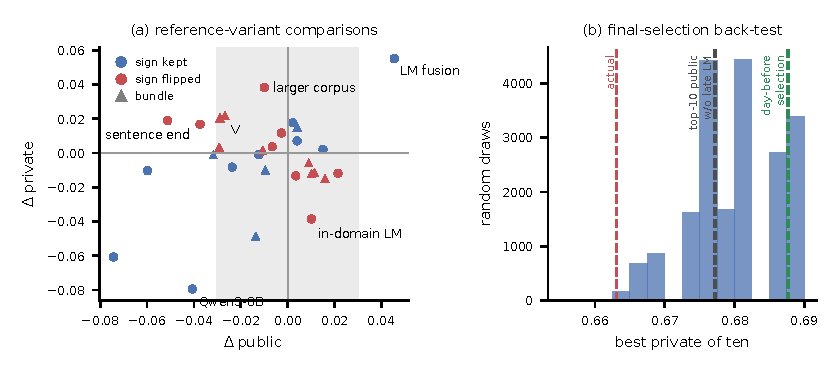
\includegraphics[width=\linewidth]{fig_pairs.pdf}
  \caption{(a) Public and private effect of each of the 30 reference--variant comparisons (one off-scale point, the sentence-context redesign at $+0.267/+0.207$, is omitted). The grey band marks absolute public effects below 0.03; red points changed sign between the splits. (b) Best private score of ten submissions drawn at random from the 60 pre-deadline submissions with public score at least 0.66 (20{,}000 draws), with our actual final selection, the ten highest public scores excluding the last-week language components, and our selection one day before the deadline.}
  \label{fig:pairs}
\end{figure}

\paragraph{Validation against public.} For eight comparisons, our component-level validation and the public score pointed in opposite directions before the private release. Private sided with validation four times and with public four times (Wilson interval for 4 of 8: 0.22--0.78). The stakes were not symmetric, however. Where validation was right, the private gains were $+0.003$ to $+0.022$: the 1\,s share, more 1\,s members, $\tau=0.3$ and the stack V. Where public was right, the losses from following validation were 0.001 to 0.010: $\tau=0.5$, the wide CNN and two word-timing strengths. On average, following validation would have gained 0.005 per decision.

These cases overlap: V contains $\tau=0.3$ and word timing, and two of the cases concern 1\,s models. During the competition we read the repeated disagreements as evidence that the proxy did not represent the test set, and we followed the public score.

\paragraph{Why small public differences were unreliable.} BAcc@10 weights each word equally, so on a split with few items per word a handful of items can move the score by 0.01--0.02. Our public scores repeat the same five-decimal values across submissions with different sentence predictions. For example, three different in-domain-LM submissions all scored 0.72001. This is consistent with a small public split, although we do not know its size.

\section{Final selection}
\label{sec:selection}

\begin{table}[t]
  \caption{Back-test of final-selection rules: best private score among ten submissions made before the deadline. The random rule uses 20{,}000 draws of ten distinct submissions from the 60 with public score at least 0.66.}
  \label{tab:select}
  \centering
  \small
  \begin{tabular}{lc}
    \toprule
    Rule & Best private \\
    \midrule
    Our actual final selection & 0.663 \\
    Ten highest public scores (8 of 10 shared with the actual selection) & 0.663 \\
    Ten highest public, excluding the last-week language components & 0.677 \\
    Ten random submissions with public $\geq 0.66$: mean (10th--90th percentile) & 0.680 (0.673--0.688) \\
    Our selection one day before the deadline (included V) & 0.688 \\
    \bottomrule
  \end{tabular}
\end{table}

Kaggle allowed ten final submissions and scores the best of them on the private split. One day before the deadline, our recorded selection deliberately mixed public-best and validation-backed submissions, including V. On the last day, after the language-side components raised the public score, the final selection replaced the validation-backed submissions with public-best ones. That moved the result from 0.6877 to 0.663. V's score would have placed it 34th on the private leaderboard of 25 October; the actual result was 44th.

Table~\ref{tab:select} and Figure~\ref{fig:pairs}b compare this with simple alternatives. Choosing the ten highest public scores gives the same 0.663. Only 0.24\% of random draws from the same 60-submission pool were as low. The pool and rules are defined in hindsight, and the pool over-represents heavily explored families, so this is a property of our submissions rather than a general result.

Our recommendations for small public splits:
\begin{enumerate}
\item Treat public differences comparable to the spread among related configurations (here about 0.03) as unreliable, especially for late changes chosen on the public split alone.
\item Reserve part of the final selection for submissions that careful validation prefers. When validation and public disagree, the downside of following validation may be small.
\item Record each submission's reference submission, so that paired effects, not only levels, can be checked afterwards.
\item Check which test rows are actually scored. Our isolated-word tuning turned out to be irrelevant.
\end{enumerate}

\section{Discussion}
For this single, deeply sampled subject, two large structural changes transferred to the private split: sentence context ($+0.207$ private) and closed-vocabulary LM fusion ($+0.055$). Many later changes moved the public and private scores by similar amounts in unrelated directions.

The language-side ideas are not refuted. Larger in-domain corpora and generic candidates improved the private score; it was the variants selected by their public scores that did not. In-session validation was an imperfect but low-risk guide. A better proxy, built from recordings outside the training sessions, would likely be the most valuable improvement. Kaggle rankings are provisional, and the organisers' verification determines the final standings.

\paragraph{Reproducibility.} The repository \url{https://github.com/kuotunyu/pnpl2026-meg-word-decoding} contains the code, the corpora, the submission export and the analysis script, and links to the checkpoints. MEG models were trained on Google Colab A100 GPUs and a local RTX 4090.

\begin{ack}
We thank the PNPL organisers for the competition and the dataset. The release of private scores for all submissions made this analysis possible. This work received no external funding; the author declares no competing interests.
\end{ack}

{\small
\begin{thebibliography}{9}
\bibitem{dascoli2025} S.~d'Ascoli et al.\ Towards decoding individual words from non-invasive brain recordings. \emph{Nature Communications}, 16, 2025. doi:10.1038/s41467-025-65499-0.
\bibitem{pnpl2026} F.~Mantegna, G.~Elvers, D.~Jayalath, G.~Landau, T.~Kim, M.~\"{O}zdogan, L.~Kurth, T.~Kwon, S.~Cho, B.~Ballyk, A.~Fung, A.~Greer, P.~Somaiya, C.~Herff, Y.~M.~Ramos, H.~Abdelhedi, K.~Jerbi, G.~Farquhar, B.~Shillingford, M.~Woolrich, O.~P.~Jones. The 2026 PNPL Competition: Word Classification and Efficient Cross-Subject Generalisation in LibriBrain100. arXiv:2609.03231, 2026.
\bibitem{radford2019} A.~Radford, J.~Wu, R.~Child, D.~Luan, D.~Amodei, I.~Sutskever. Language models are unsupervised multitask learners. OpenAI technical report, 2019.
\bibitem{qwen35} Qwen Team. Qwen3.5-9B. Model card, \url{https://huggingface.co/Qwen/Qwen3.5-9B}, 2026.
\end{thebibliography}
}

\appendix
\section{All reference--variant comparisons}
\label{app:pairs}
S: one documented change; B: several changes at once. Validation as in Table~\ref{tab:pairs}; it is component-level and was recorded before the private release, though sometimes after the public result. Some reference submissions were created after their variant, as matched controls. Generated by \texttt{analysis/analyze\_lb.py} and \texttt{make\_tables.py} from \texttt{analysis/data/submissions\_raw.csv}.

\noindent\resizebox{\linewidth}{!}{\begin{tabular}{lllcrrc}
\toprule
Change & Reference & Variant & & $\Delta$ pub. & $\Delta$ priv. & Val. \\
\midrule
    sentence-context model (redesign) & \texttt{sub\_v1} & \texttt{sub\_c1} & B & $+0.267$ & $+0.207$ & n/a \\
    closed-vocab LM fusion (PMI) & \texttt{sub\_c5} & \texttt{sub\_c5\_lmpmi05} & S & $+0.045$ & $+0.055$ & $+$ \\
    N-best hard marginals instead of soft PMI & \texttt{sub\_c5\_lmpmi05} & \texttt{sub\_c5\_lm05} & S & $-0.074$ & $-0.061$ & n/a \\
    Qwen3-8B instead of GPT-2 & \texttt{final\_gpt2} & \texttt{final\_qwen3\_8b} & S & $-0.041$ & $-0.079$ & $-$ \\
    3 s window ensemble & \texttt{final\_gpt2} & \texttt{finalW\_gpt2} & B & $+0.016$ & $-0.015$ & n/a \\
    LM strength calibration (+ GPT-2-medium) & \texttt{finalW\_gpt2} & \texttt{finalW\_calib2} & S & $+0.003$ & $-0.013$ & n/a \\
    sentence prior correction $\tau{=}0.5$ & \texttt{finalW\_calib2} & \texttt{finalW\_calib2\_t0.5} & S & $-0.012$ & $-0.001$ & $+$ \\
    higher 1 s share & \texttt{finalW\_calib2\_iso14} & \texttt{finalY\_calib2\_t0} & B & $-0.029$ & $+0.003$ & $+$ \\
    self-training round 1 & \texttt{finalW\_calib2\_iso14} & \texttt{final\_P1} & S & $+0.015$ & $+0.002$ & n/a \\
    LM fusion after self-training & \texttt{final\_P1noLM} & \texttt{final\_P1} & S & $+0.022$ & $-0.012$ & n/a \\
    self-training round 2 (all replaced) & \texttt{final\_P1} & \texttt{final\_P2} & B & $-0.010$ & $-0.010$ & n/a \\
    sentence-end LM term & \texttt{final\_P1} & \texttt{final\_P1eos} & S & $-0.051$ & $+0.019$ & n/a \\
    larger diverse ensemble & \texttt{final\_P1} & \texttt{final\_B2} & B & $+0.004$ & $+0.015$ & n/a \\
    12-layer + wide-CNN members & \texttt{final\_B2} & \texttt{final\_B5} & B & $+0.012$ & $-0.012$ & n/a \\
    all members self-trained (one teacher) & \texttt{final\_B2} & \texttt{final\_C} & B & $-0.014$ & $-0.049$ & n/a \\
    more 1 s members & \texttt{final\_B5} & \texttt{final\_B6a} & B & $-0.029$ & $+0.021$ & $+$ \\
    wide CNN instead of 12-layer & \texttt{final\_B5} & \texttt{final\_F1} & B & $-0.032$ & $-0.001$ & $+$ \\
    sentence prior correction $\tau{=}0.3$ & \texttt{final\_B5i} & \texttt{final\_B5i\_t0.3} & S & $-0.037$ & $+0.017$ & $+$ \\
    word-timing evidence $\beta{=}0.5$ & \texttt{final\_B5i} & \texttt{final\_B5d05} & S & $-0.060$ & $-0.010$ & $+$ \\
    word-timing evidence $\beta{=}1.0$ & \texttt{final\_B5i} & \texttt{final\_B5d10} & S & $-0.024$ & $-0.008$ & $+$ \\
    input rescaling & \texttt{final\_B5i} & \texttt{final\_B5irs} & S & $-0.007$ & $+0.004$ & n/a \\
    validation-motivated stack V & \texttt{final\_B5i} & \texttt{final\_V} & B & $-0.027$ & $+0.022$ & $+$ \\
    lr-fixed deep members & \texttt{final\_B5i} & \texttt{final\_B8b} & B & $-0.011$ & $+0.002$ & n/a \\
    in-domain LM (807 sentences) & \texttt{final\_B5i} & \texttt{final\_B5i\_L1} & S & $+0.010$ & $-0.038$ & n/a \\
    in-domain LM, 3-seed mixture & \texttt{final\_B5i} & \texttt{final\_B5i\_L1avg} & B & $+0.010$ & $-0.012$ & n/a \\
    in-domain corpus 807 $\to$ 1,368 & \texttt{final\_B5i\_L1} & \texttt{final\_B5i\_L3} & S & $-0.010$ & $+0.038$ & n/a \\
    in-domain corpus 807 $\to$ 2,103 (IN1) & \texttt{final\_B5i\_L1\_IN1} & \texttt{final\_IN1\_Q\_llm\_plus} & S & $+0.002$ & $+0.018$ & n/a \\
    in-domain corpus 2,103 $\to$ 3,742 (IN1) & \texttt{final\_IN1\_Q\_llm\_plus} & \texttt{final\_IN1\_Q\_big} & S & $+0.004$ & $+0.007$ & n/a \\
    generic candidates, $\lambda{=}0.15$ & \texttt{final\_IN1\_Q\_llm\_plus} & \texttt{final\_IN1Qp\_SC0.15} & S & $-0.003$ & $+0.012$ & n/a \\
    candidate decoding (guided pool + LM prior) & \texttt{final\_IN1\_Q\_llm\_plus} & \texttt{final\_IN1Qp\_SCGL\_b0.5} & B & $+0.009$ & $-0.006$ & n/a \\
\bottomrule
\end{tabular}
}

\end{document}
